\documentclass{article}
\usepackage{tikz}
\usepackage{mathpazo}
\usepackage{xcolor}

\usepackage{verbatim}

\newcounter{row}
\newcounter{col}

\edef\puzzlescale{1.2}
\edef\numrows{4}

  \addtolength{\itemsep}{-0.5\baselineskip}

\newcommand\setrow[\numrows]{
  \setcounter{col}{1}
  \foreach \n in {#1, #2, #3, #4} {
    \edef\x{\value{col} - 1}
    \edef\y{1 + \numrows - \value{row}}
    \node[anchor=north west,scale=0.75*\puzzlescale] at (\x, \y) {\n};
    \stepcounter{col}
  }
  \stepcounter{row}
}

\newcommand\boldh[3]{
  \edef\y{\numrows-#1}
  \edef\x{#2}
  \edef\z{\x + #3}
  \draw[very thick] (\x, \y) -- (\z, \y);
}

\newcommand\boldv[3]{
  \edef\y{\numrows-#1}
  \edef\x{#2}
  \edef\z{\y - #3}
  \draw[ultra thick] (\x, \y) -- (\x, \z);
}

\definecolor{shadegray}{gray}{0.75}

\newcommand\shadebox[2]{
  \edef\y{\numrows-#1}
  \edef\x{#2}
  \fill[shadegray] (\x, \y) rectangle (\x+1,\y-1);
}

\begin{document}

\begin{center}
  \large \textbf{John Doe and Jane Dee}

  Table ?
\end{center}

Hello, friends! 
Your table is named for one of the four Shakespeare plays listed
below.  To find which, solve the KenKen puzzle, and the number in the
shaded box will indicate your table.  Or, just identify which
play includes the quoted line.  Have fun!

\medskip

\begin{minipage}[top]{0.5\textwidth}
  \textit{To be, or not to be?}
  \begin{enumerate}
  \item Hamlet
  \item A Midsummer Night's Dream
  \item Romeo and Juliet
  \item Twelfth Night
  \end{enumerate}
\end{minipage}
%
\begin{minipage}[top]{0.5\textwidth}
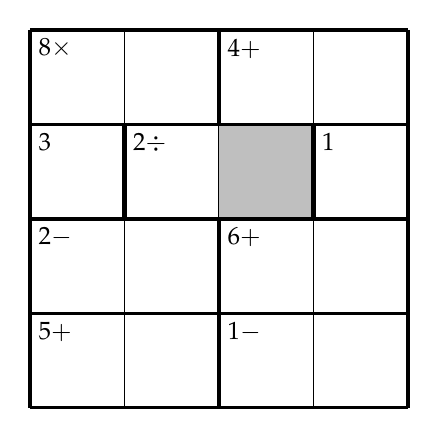
\begin{tikzpicture}[scale=\puzzlescale]

  \begin{scope}

    \shadebox{1}{2}
    
    \draw (0, 0) grid (4, 4);
    \boldh{0}{0}{4}
    \boldh{1}{0}{4}
    \boldh{2}{0}{4}
    \boldh{3}{0}{4}
    \boldh{4}{0}{4}
    \boldv{0}{0}{4}
    \boldv{1}{3}{1}
    \boldv{1}{1}{1}
    \boldv{0}{2}{1}
    \boldv{2}{2}{2}
    \boldv{0}{4}{4}

    \setcounter{row}{1}
    \setrow {$8\times$} {} {$4+$} {}
    \setrow {$3$} {$2\div$} {} {$1$}
    \setrow {$2-$} {} {$6+$} {}
    \setrow {$5+$} {} {$1-$} {}
    
    % \node[anchor=center] at (0.5*\numrows, -0.5) {Ken Ken};
  \end{scope}

\end{tikzpicture}
\end{minipage}
%

Rules for KenKen: Fill in the boxes with the numbers 1 through 4, with
each number appearing exactly once in every row and column.  Each
``cage'' (set of boxes outlined in bold) has a target number
and mathematical operation in the top-left; combining each
number in the cage with the operation must result in the target.
\textit{Hint}: For cages with no operation, just fill in the
  target number.

\begin{center}
\it Solutions may be found on the inside of the card.
\end{center}

\end{document}
